\subsection{M4 Upper Bound}
\begin{figure}[h]
	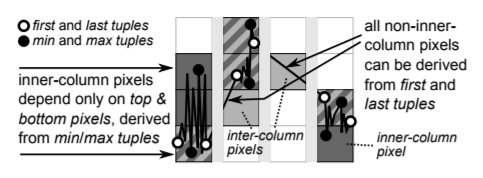
\includegraphics[width=0.5\textwidth]{th1}
	\caption{Illustration of Theorem 1}   
	\label{fig:3}
\end{figure}
The question is common to be asked, whether selecting only four extreme tuples from each group provide error free visualization. The authors of the paper provide some proofs on the upper bound on the number of tuples required for error free visualization. The authors prove two theorems to show that the four extreme tuples are sufficient enough for error free visualization of time series data. 
\begin{theorem}
	Any two-color line visualization of an arbitrary
	time series T is equal to the two-color line visualization
	of a time series T'
	that contains at least the
	four extrema of all groups of the width-based grouping
	of T, i.e., $vis_{wh}(G_{M4}(T)) = vis_{wh}(T)$.
\end{theorem}
The illustration of theorem 1 is given Figure \ref{fig:3}.  The authors provide a detailed proof in the paper.

\begin{theorem}
	There exists an error-free two-color line visualization
	of an arbitrary time series T, based on a
	subset $T'$ of $T$, with $|T'| \leq 4 · w$.
\end{theorem}